% This program is free software: you can redistribute it and/or modify it under the terms of the GNU General Public License as published by the Free Software Foundation, either version 3 of the License, or (at your option) any later version.
%
% This program is distributed in the hope that it will be useful, but WITHOUT ANY WARRANTY; without even the implied warranty of MERCHANTABILITY or FITNESS FOR A PARTICULAR PURPOSE. See the GNU General Public License for more details.
%
% You should have received a copy of the GNU General Public License along with this program. If not, see <https://www.gnu.org/licenses/>.

% This program is free software: you can redistribute it and/or modify it under the terms of the GNU General Public License as published by the Free Software Foundation, either version 3 of the License, or (at your option) any later version.
%
% This program is distributed in the hope that it will be useful, but WITHOUT ANY WARRANTY; without even the implied warranty of MERCHANTABILITY or FITNESS FOR A PARTICULAR PURPOSE. See the GNU General Public License for more details.
%
% You should have received a copy of the GNU General Public License along with this program. If not, see <https://www.gnu.org/licenses/>.

\documentclass[10pt,presentation]{beamer}

\usetheme[progressbar=frametitle, numbering=fraction, background=dark]{metropolis}
\usepackage{appendixnumberbeamer}

\usepackage{booktabs}
\usepackage[scale=2]{ccicons}

\usepackage{hyperref}
\usepackage{multimedia}

\usepackage{enumerate}
\usepackage[skip=2pt]{caption}

\usepackage{dirtytalk}
\usepackage{multimedia}
\usepackage[outputdir=build]{minted}

\usepackage{tikz}
\usepackage{tikzducks}
\usepackage{bookmark}

% https://tex.stackexchange.com/questions/152392/date-format-yyyy-mm-dd
\usepackage[yyyymmdd]{datetime}
\renewcommand{\dateseparator}{--}

% Copied from https://github.com/matze/mtheme/blob/master/source/beamerinnerthememetropolis.dtx
\setbeamertemplate{title page}{
  \begin{minipage}[b][\paperheight]{\textwidth}
    \vfill%
    \ifx\inserttitle\@empty\else\usebeamertemplate*{title}\fi
    \ifx\insertsubtitle\@empty\else\usebeamertemplate*{subtitle}\fi
    \usebeamertemplate*{title separator}
    \ifx\inserttitlegraphic\@empty\else\usebeamertemplate*{title graphic}\fi
    \ifx\beamer@shortauthor\@empty\else\usebeamertemplate*{author}\fi
    \ifx\insertdate\@empty\else\usebeamertemplate*{date}\fi
    \ifx\insertinstitute\@empty\else\usebeamertemplate*{institute}\fi
    \vfill
    {\tiny Copyright (C) 2023 Jamal Bouajjaj under GPLv3} \par
    \vspace*{5mm}
    \vspace*{1mm}
  \end{minipage}
}

\setbeamertemplate{title graphic}{
  \vbox to 0pt {
    \vspace*{0em}
    \inserttitlegraphic%
  }%
  \nointerlineskip%
}

\titlegraphic{\hfill \begin{tikzpicture}[scale=0.75]
\duck[magichat,magicwand,magicstars=blue!60!white,squareglasses=blue!50!black]
\end{tikzpicture}}

\newenvironment{Figure}
  {\par\medskip\noindent\minipage{\linewidth}\centering}
  {\endminipage\par\medskip}

\newcommand\Wider[2][3em]{%
\makebox[\linewidth][c]{%
  \begin{minipage}{\dimexpr\textwidth+#1\relax}
  \raggedright#2
  \end{minipage}%
  }%
}


\usepackage{media9}
\usepackage{multicol}

\title{Lecture \#15: Copyright}
\date{\today}
\author{Presented by Jamal Bouajjaj}
\institute{For University of New Haven's Fall 2023 CSCIxx51 Course}

% From https://tex.stackexchange.com/questions/66519/make-each-frame-not-slide-appear-in-the-pdf-bookmarks-with-beamer
\makeatletter
\apptocmd{\beamer@@frametitle}{\only<1>{\bookmark[page=\the\c@page,level=3]{#1}}}%
% {\message{** patching of \string\beamer@@frametitle succeeded **}}%
% {\message{** patching of \string\beamer@@frametitle failed **}}%
\makeatother

\begin{document}

\maketitle

\begin{frame}{Intro}
  Let's say you make some form of art or work, like a book, painting, or code?\pause

  In a zero-law world, what is stopping me from taking that work and re-publishing it? \pause

  Wouldn't it be nice if you owned the work you made?
\end{frame}

\begin{frame}{Copyright}
  This is where we have copyright, which is
  \begin{quote}
  a type of intellectual property that gives its owner the exclusive right to copy, distribute, adapt, display, and perform a creative work, usually for a limited time.\footnote{\url{https://en.wikipedia.org/wiki/Copyright}}
  \end{quote}
  \begin{columns}[onlytextwidth,T]
  \column{0.8\linewidth-5mm}
  Almost every country has and enforces laws regarding protecting the copyright of a work. \pause

  Note that \textit{ideas} cannot be copyrighted, only the work itself. \pause

  TL;DR: When you make a creative work, you have exclusive right over that work by law.

  \column{0.2\textwidth}
  \center 
\includegraphics[width=\textwidth]{eimg/copyrightSym.png}
  \end{columns}
\end{frame}

\begin{frame}{Time}
  So if you made something, can you own the copyright on it forever??\pause

  Ehhh....no\pause

  Copyright law set a duration before the work becomes into the \textit{Public Domain}. The idea is to have society build upon copyright work after the author benefits from the exclusive right.

  The time has been extended (here in the US) many times thanks to the Disney corporation (think Mickey Mouse)`.
\end{frame}

\begin{frame}{Time Extensions in the US}
  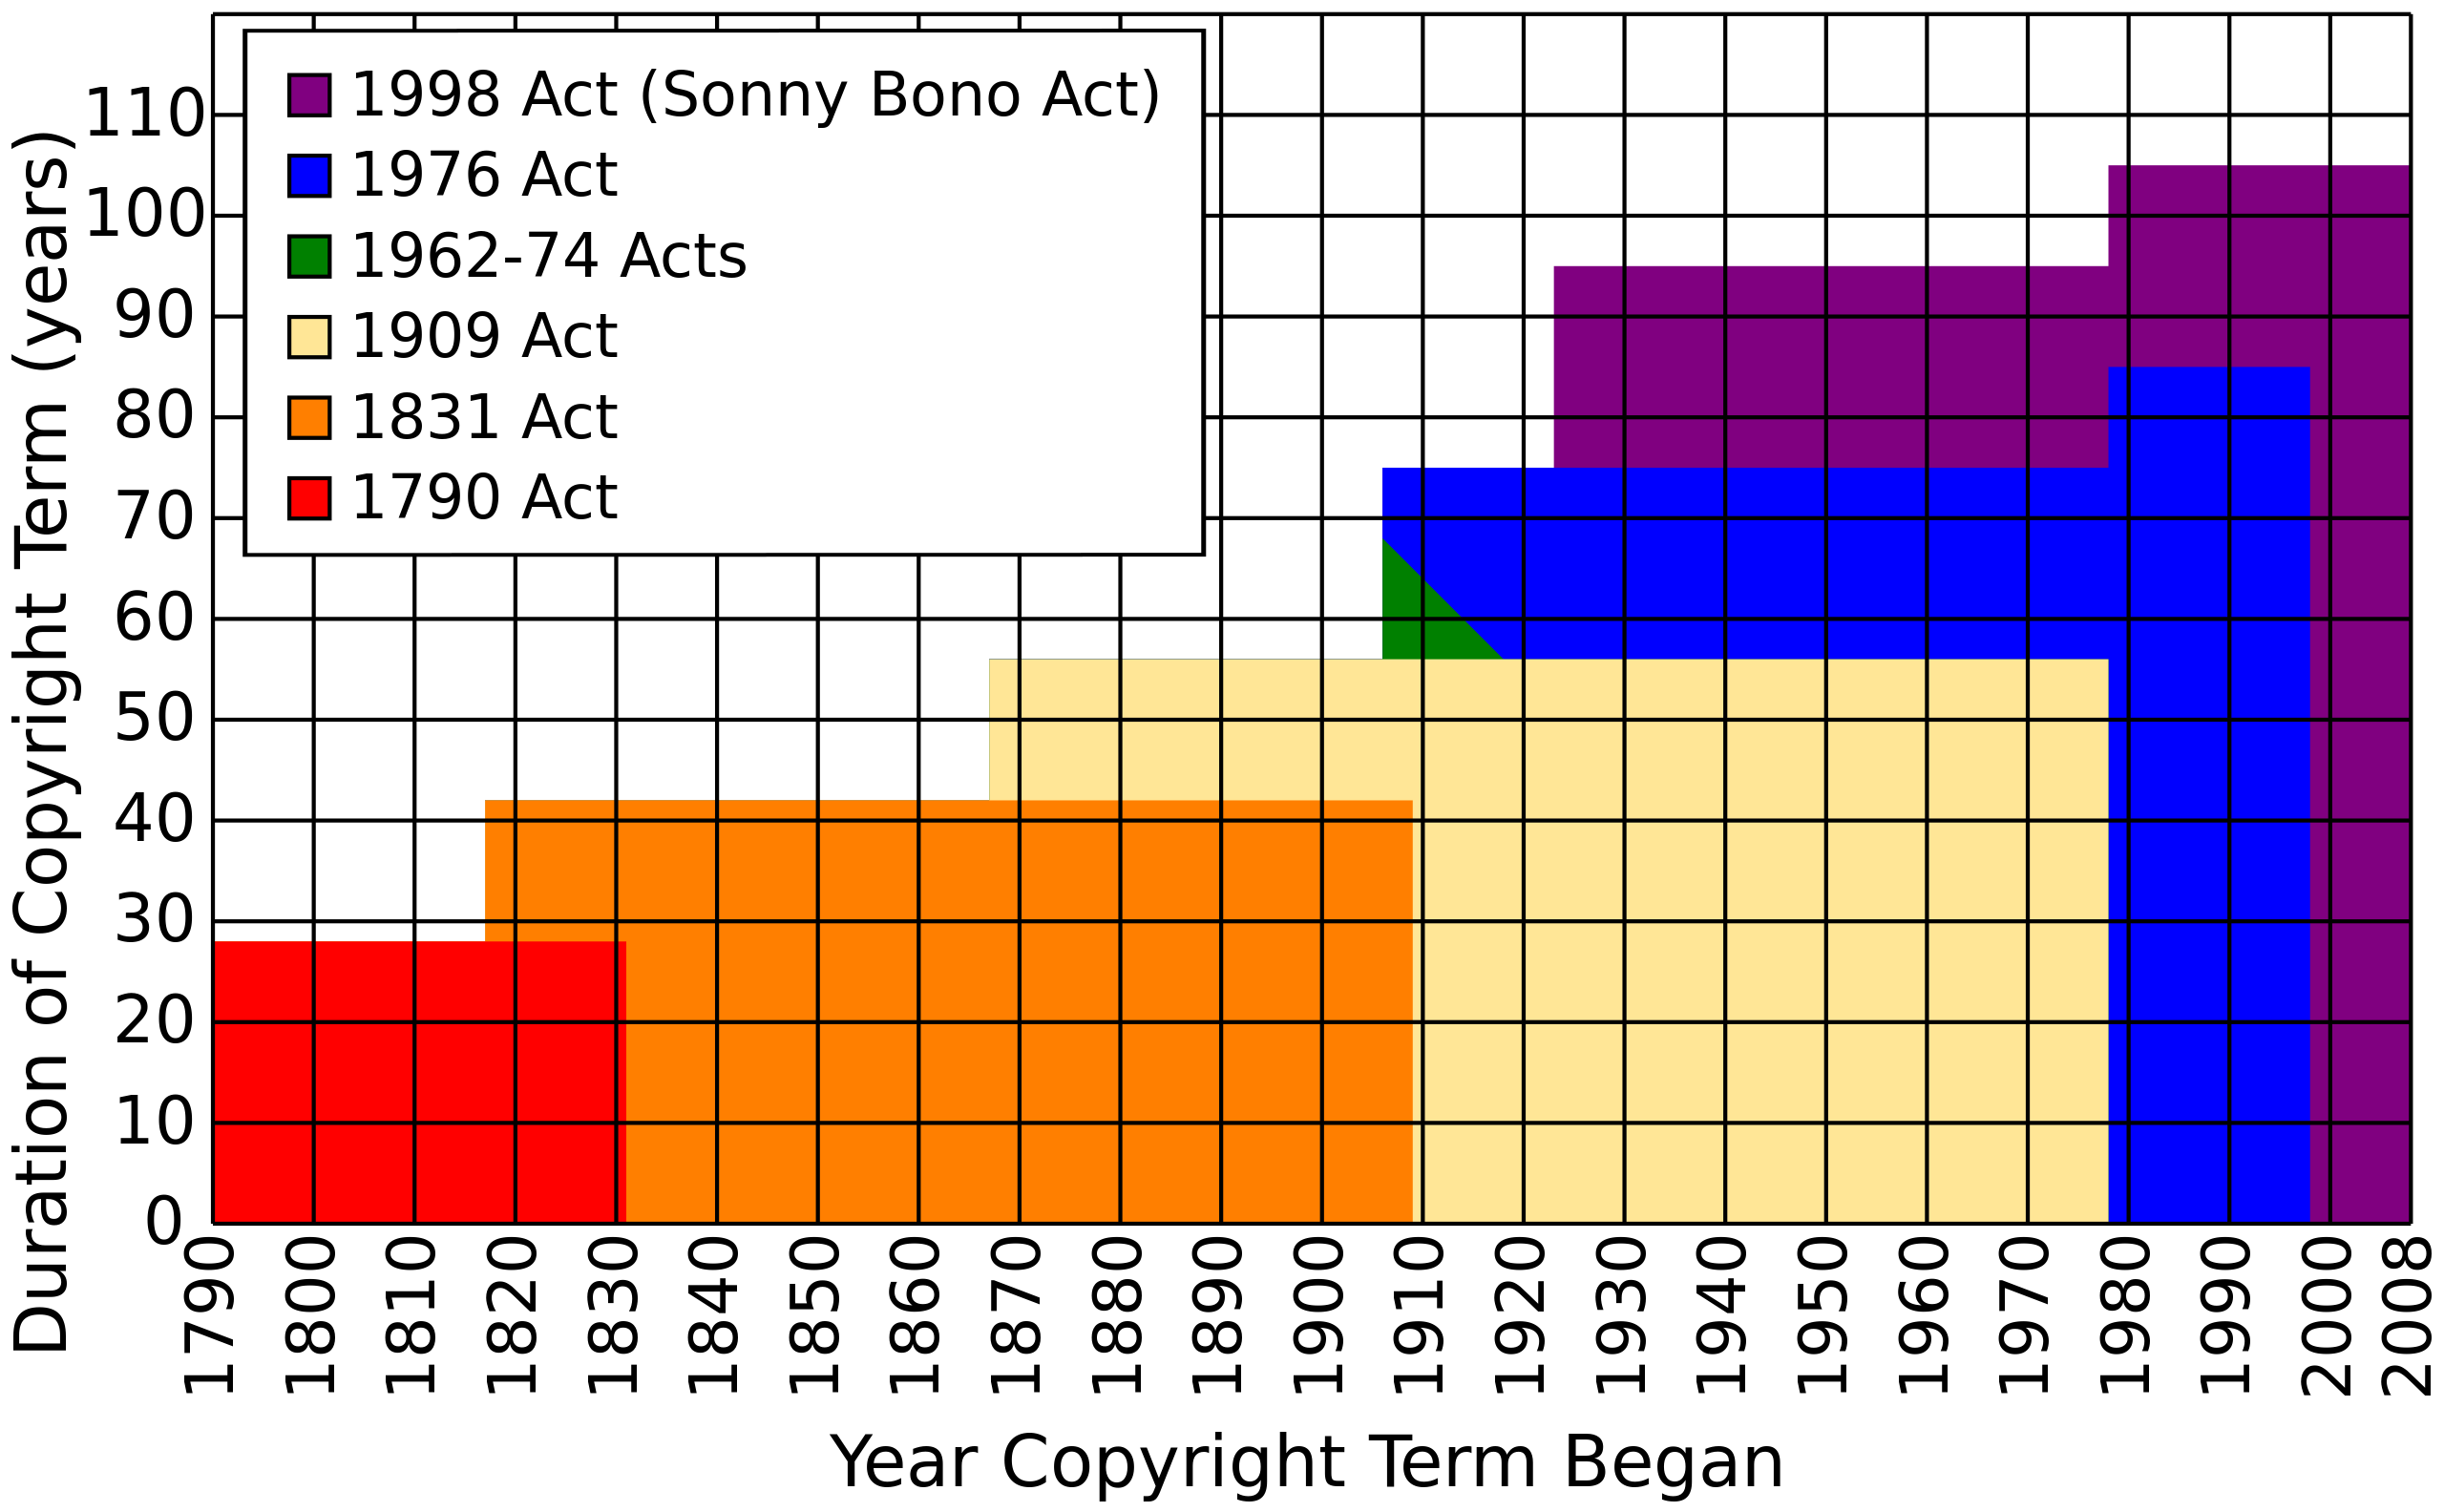
\includegraphics[width=\textwidth]{eimg/TomBell'sgraphshowingextensionofUScopyrighttermovertime.png}
\end{frame}

\begin{frame}{Time Extensions in the US}
  The Public Domain are all creative works with no exclusive IP rights. This is where all copyrighted works eventually go.
\end{frame}

\begin{frame}{Time Extensions in the US}
\begin{columns}[onlytextwidth,T]
  \column{0.8\linewidth-5mm}
    The Public Domain are all creative works with no exclusive IP rights. This is where all copyrighted works eventually go.
  \column{0.2\textwidth}
  \center 
\includegraphics[width=\textwidth]{eimg/PDSymbol.png}
  \end{columns}
\end{frame}

\begin{frame}{What if...free}
  But can you use your copyright power to ensure \textit{FREEDOM} for those who use your creative works?\pause

  What if you want to put your work out publicly for humanity to use, but with some restrictions? \pause
\begin{columns}[onlytextwidth,T]
  \column{0.8\linewidth-5mm}
  The answer is yes, as copyright gives the author exclusive rights over the work, including the right to just publish it as public domain, or publish it freely with restrictions. You can use that power to ensure your copyright work is published freely, and nobody is able to use it without the ability modify, share, copy, or redistribute (under the same or similar license) your work.

  This concept is known as copyleft.
  \column{0.2\textwidth}
  \center 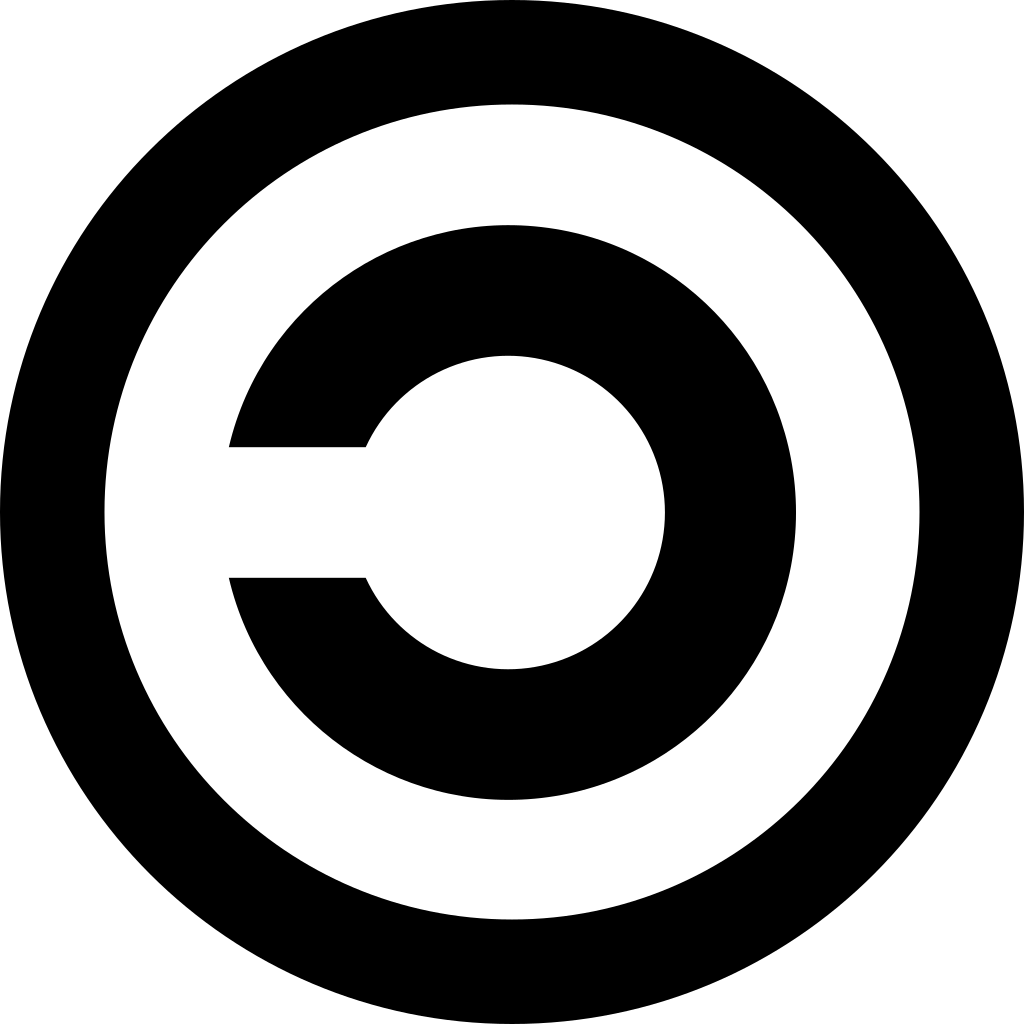
\includegraphics[width=\textwidth]{eimg/CopyleftSym.png}
  \end{columns}
\end{frame}

\begin{frame}{Distribution}
  Most licenses (if not all) only apply when you \textit{distribute} the works. So if you are using a copyleft work for an internal non-distributed work, you may not need to follow it's license clauses (see GPL for example).
\end{frame}


\begin{frame}{CC Licenses}
  For generate creative works, the \textit{Creative Commons license} are several licenses that you can use in your work. The license enables free usage of your work.

  There are restrictions in the different licenses which you can choose for your work (single or in combination), which includes:
  \begin{itemize}
    \item (BY) Attribution
    \item (SA) Share-Alike (Required for works to be considered copyleft)
    \item (NC) Non-Commercial
    \item (ND) Non Derivative Works
  \end{itemize}

  There is also a CC0 license, which is just a license to put your work in the public domain.
\end{frame}

\begin{frame}{Software License: GPL}
  \footnotesize
  Somebody, in around the 1990s, wanted to guarantee the following software freedoms to the users\footnote{\url{https://www.gnu.org/philosophy/free-sw.html}}
  \begin{itemize}
    \item The freedom to run the program as you wish, for any purpose (freedom 0).
    \item The freedom to study how the program works, and change it so it does your computing as you wish (freedom 1). Access to the source code is a precondition for this.
    \item The freedom to redistribute copies so you can help others (freedom 2).
    \item The freedom to distribute copies of your modified versions to others (freedom 3). By doing this you can give the whole community a chance to benefit from your changes. Access to the source code is a precondition for this.
  \end{itemize}\pause

  That person was Richard Stallman (also the maker of the GNU project and a contributor to GCC), and he formed the GPL license (GNU General Public License).
\end{frame}

\begin{frame}{GPL}
  GPL is the one of the list restrictive copyleft licenses. It guarantees the freedoms by ensuring that
  \begin{itemize}
    \item Any GPL source code is accessible freely to the user
    \item Any published result of a modified GPL source code must also have the source code available to the users
    \item Any published software built on top of GPL code, even if there was no modifications to the GPL code, must also be published under the GPL licence.
  \end{itemize} \pause
  This is important, as you may not be able to just use GPL code in your (or company's) code due to the last clause above.\pause

  Did you know that these slides are under a GPLv3 license? (Source code is on Github, link on Canvas)
\end{frame}

\begin{frame}{LGPL}
  Lesser-GPL is a version of GPL which removes the restriction of requiring the software using GPL licensed code to publish their own code, which is suitable for some libraries.
\end{frame}

\begin{frame}{MIT}
  The MIT license is one of the most permissive permissive licenses, the only clauses being attribution and lack of warrantee.

  MIT is not copyleft, as someone can take MIT code, modify it, and publish the modification without releasing the source code.
\end{frame}

\begin{frame}{Lots More}
  There are a lot of software licences out there, with different clauses and varieties.

  If you are using some software (such as a library) in your company's code, check the license of the works.

  If you are making software, you have the freedom to keep the code as "All Rights Reserved", or use that power to ensure software freedom to the extent you want.
\end{frame}

\end{document}
